\chapter{IMPLEMENTATION}
\begin{spacing}{1.5}
The proposed system currently addresses the composition of RESTful web services that represent resources using the JavaScript Object Notation (JSON). The system expexts the services to return results to API queries as JSON objects and composes them as per the user specification. Extension of the same idea can enable the composition of XML based RESTful services.The system also includes an RDF conversion module that performs the automatic conversion process from Microformat annotations to RDF.

The system uses a web UI developed in HTML, JavaScript as the frontend for reading user input. The requests are handled by a server program developed in node.js that accepts requests from multiple client machines and handles them asynchronously. The server program acts as a proxy and is developed to enable the system to handle high volumes of client traffic. The server does the bulk of orocessing and also allows multiple cross domain HTTP calls with ease, which would otherwise be not possible with a client side implementation because of the same origin policy enforced by the modern web browsers. The basic architecture of the system is as illustratred in Figure: \ref{fig:architecture}

\begin{figure}
        \centering
        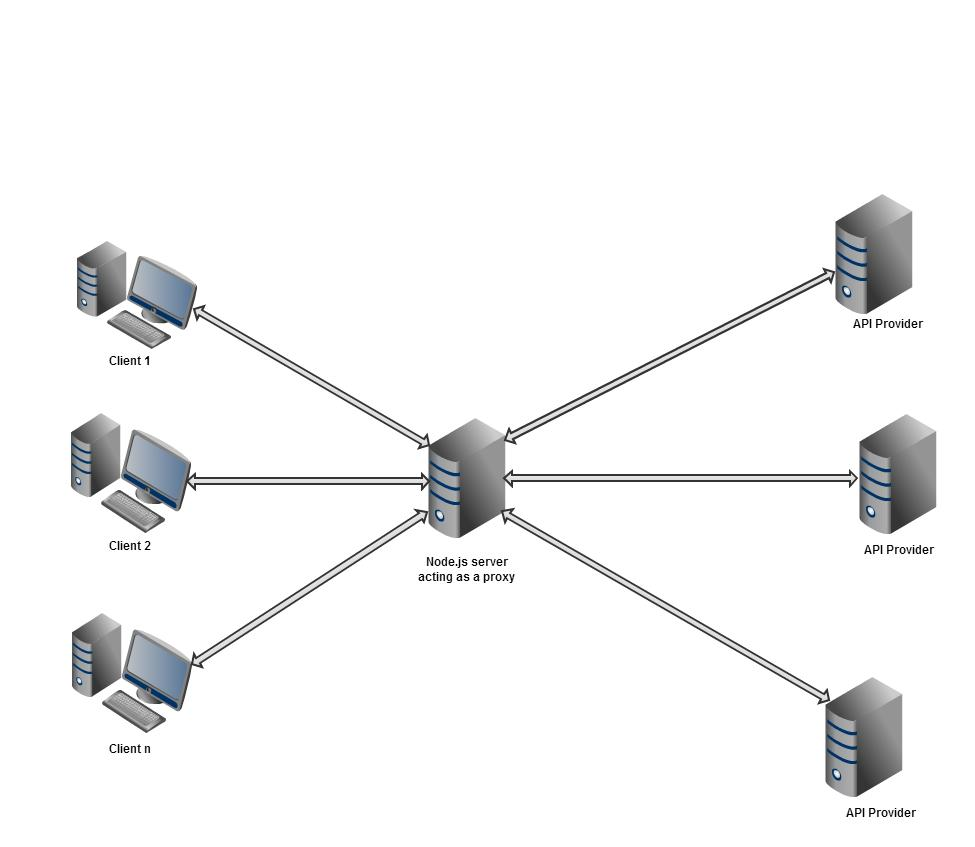
\includegraphics[scale=0.3]{images/Architecture.jpg}
        \caption{System architecture }
        \label{fig:architecture}
\end{figure}

The system uses a parser module to parse the DOM tree of the annotated API Documentation page and extract the information embedded in it. Based on users input of which APIs to use for composition, the server fetches each of the required annotated API documentation pages and parses them. Based on the information extracted from DOM tree, the web UI presented to the user is populated with a set of API operations that the system identifies and that can be composed. A workbench is presented to the user and a drag-drop based user interface enables the him/her to graphically descipbe the required composition of web services. Once the mashup is graphical design of the mashup is complete and user submits it, information from the design is converted into an abstract internal representation that is passed to the server. The server now invokes the reqired API calls asynchronouly and composes them as required and produces an HTML formatted output which is the required mashup. The HTML output is then served back to the client system for the user. The interaction flow in the system is illustrated in Figure: \ref{fig:sequence}

\begin{figure}
        \centering
        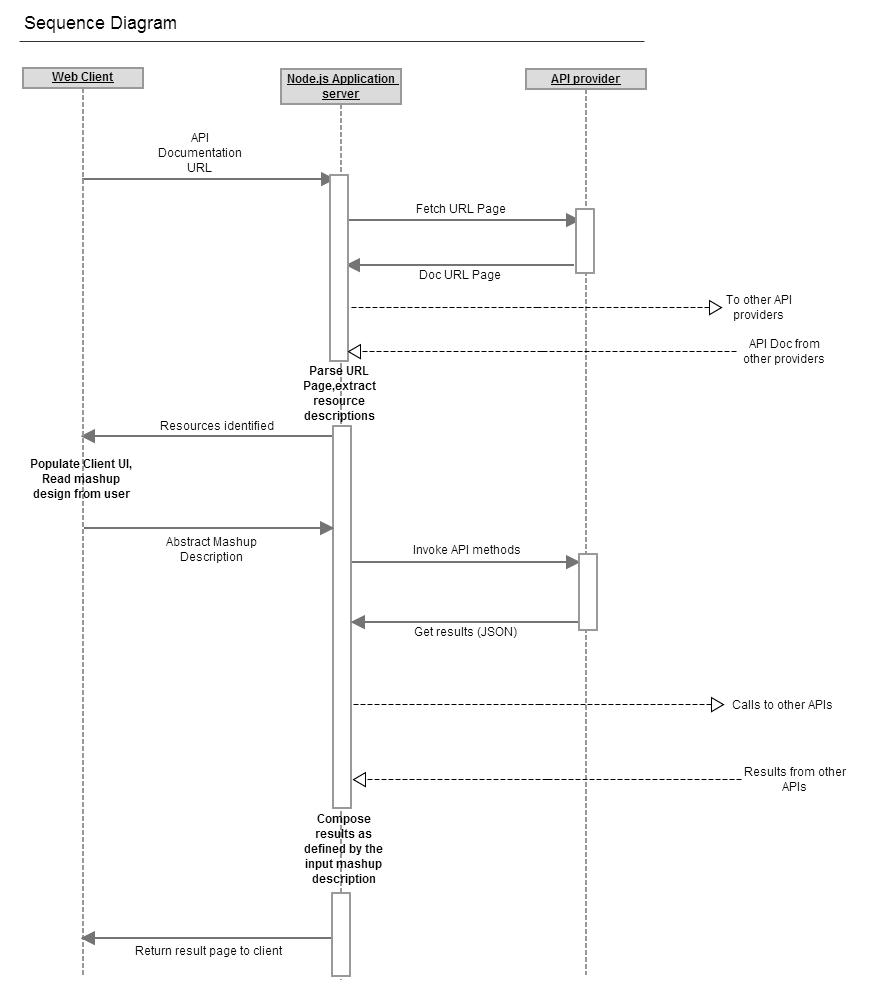
\includegraphics[scale=0.5]{images/smashup_sequence.jpg}
        \caption{Interaction flow sequence}
        \label{fig:sequence}
\end{figure}

\section{Server side Implementation}
The architecture of the server is as illustrated in Figure: \ref{fig:serverarch}.Server primarily deals with providing three services:
\begin{enumerate}

\item{\bf Parsing API Documentation HTML}: Client side provides a URL to an annotated API Documentation HTML page. The server fetches the required documentation page and passes the HTML DOM to the parser module {\it(hrestsparser)}. The parser generates a JSON description of the annotated resources which is then passed to the client to populate the client UI. The parser uses XPath for the traversal of the DOM tree and hence platform neutral.

\begin{figure}
        \centering
        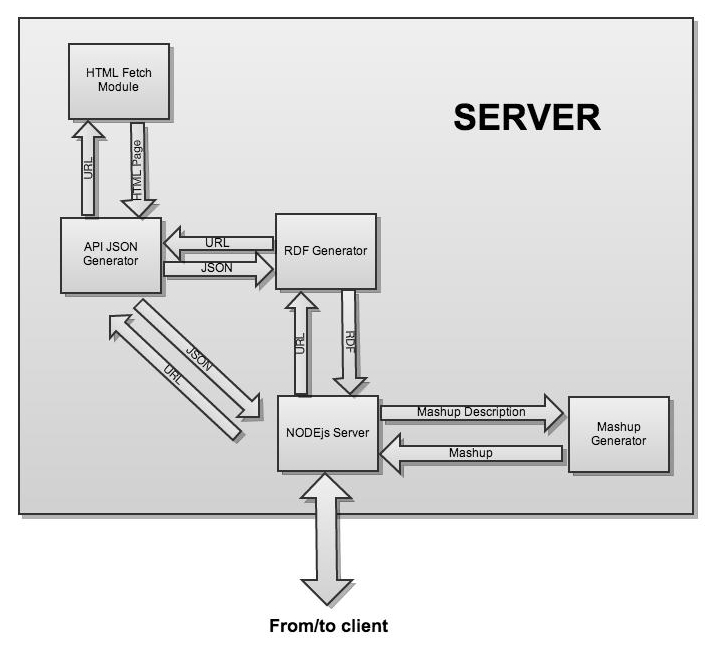
\includegraphics[scale=0.4]{images/Server_Architecture.jpg}
        \caption{Server Architecture}
        \label{fig:serverarch}
\end{figure}

\item{\bf RDF Generation}: Client passes a URL to the server. The page is fetched by the RDF generator module. The page is parsed by the hRESTS parser module to produce the output JSON. The {\it produced-by} - {\it consumed-by} relations in the annotated page forms a graph of resources each of which is required for the generation of the RDF description. The RDF generator module recursively traverses the producer-consumer graph and fetches each of the required resources upto some arbitrary level of nesting. Once the resource fetching is done RDF can be generated.

\item{\bf Request handling and mashup generation}: The user specifeis the required composition of services graphically in the client workbench. An abstract description of the required mashup is generated at the client and is passed to the server as a JSON object. The server makes the required API invocations to fetch each of the resources to be composed into the final mashup. The description JSON is parsed and the result resources are composed as specified producing an HTML output which is then served to the client system.
\end{enumerate}

\section{Client side Implementation}
Client provides a simple drag and drop based user interface for mashup design. The elements in the UI are populated from the contents of the API documantations passed to the server. The different API calls can be simply dragged and dropped to the workbench and the inputs and outputs can be piped to one another by graphical connectors.

Client uses two basic data structures which are simple JSON objects.
\begin{itemize}
\item{\bf docjsons}: An array of JSON description of all APIs loaded into the workbench
\item{\bf attributearray}: An associative array indexed using the ID of the API call used ( one for each widget used in the workbench). It has the following components:
\begin{enumerate}
\item{\it jindex}: Index of document JSON in array of JSONs.
\item{\it apiindex}: Index of the particular API used in this JSON
\item{\it isStartNode}: True if there are no inputs piped into this node ,i.e, this node is a start point in the mashup design with inputs from the user and not from other API calls.
\item{\it method}: HTTP method selected by the user.
\item{\it inputs}: An associative array of inputs indexed by attribute name.
\item{\it outputs}: An associative array of outputs indexed by attribute name.
\item{\it headers}: An associative array containing the headers to be passed (if required) with an API call, indexed by attribute name.
\end{enumerate}

Each element in the inputs array has two attributes :
\begin{itemize}
\item{\it value}: Value of the attribute or null.
\item{\it link}: Null or a tuple (id of the producer API call,name of the attribute producing it)
\end{itemize}

Each element in the outputs array has a single attribute:
\begin{itemize}
\item{\it link}: Null or a tuple (id of the consumer API call,name of the attribute that consumes it)
\end{itemize}

\end{itemize}

The link attributes forms a logical graph of the way in which the different service calls are composed. An abstract representation of the mashup is created by traversing the graph. The traversal is done by using a simple modification to the Depth First Search technique. The abstract representation is a JSON object which represents the initiation sequence for the API calls. This is then passed to the server.

\section{Tools and Technologies}

\subsection{Resource Description Framework (RDF)}
RDF is a W3C standard\cite{rdf} for modeling and sharing distributed knowledge based on a decentralized open-world assumption. Any knowledge about anything can be decomposed into triples (3-tuples) consisting of subject, predicate, and object; essentially, RDF is the lowest common denominator for exchanging data between systems.RDF is designed to be read and understood by machines.It is normally written in XML.RDF is a part of W3C's semantic web activity.

What makes RDF suited for distributed knowledge is that RDF applications can put together RDF files posted by different people around the Internet and easily learn from them new things that no single document asserted. It does this in two ways, first by linking documents together by the common vocabularies they use, and second by allowing any document to use any vocabulary. This flexibility is fairly unique to RDF.

The use cases of RDF, as described by Richard Cyganiak on the W3C's Semantic Web activiy is as follows:
\begin{itemize}
\item{to integrate data from different sources without custom programming.}
\item{to offer your data for re-use by other parties.}
\item{to decentralize data in a way that no single party {\it owns} all the data.}
\end{itemize}


RDF describes resources as tripples with subject as the identifier of the resource,predicate as the property and object as the value of the property.The linking structure of RDF forms a directed, labeled graph, where the edges  represent the named link between two resources, represented by the graph nodes.This graph view is the easiest possible mental model for RDF and is often used in easy-to-understand visual explanations.


\subsection{Bootstrap Framework}
Bootstrap is a front-end toolkit developed by twitter for rapidly developing web applications\cite{bootstrap}.It contains HTML and CSS-based design templates
for typography, forms, buttons, charts, navigation and other interface components, as well as optional JavaScript extensions. At its core, Bootstrap is just CSS, but it's built with Less, a flexible pre-processor that offers much more power and flexibility than regular CSS. With Less, it gains a range of features like nested declarations, variables, mixins, operations, and color functions. Additionally, since Bootstrap is purely CSS when compiled via Less, two important benefits are observed:

First, Bootstrap remains very easy to implement; just drop it in your code and go. Compiling Less can be accomplished via Javascript, an unofficial Mac application, or via Node.js.

Second, once complied, Bootstrap contains nothing but CSS, meaning there are no superfluous images, Flash, or Javascript.All that remains is simple and powerful CSS for your web development needs.

We used bootstrap for cross browser compatibility.The front end of the client side is built on top of bootstrap framework.

\subsection{JSPlumb}
jsPlumb provides a means for a developer to visually connect elements on their web pages.It uses Bezier curve functions for plotting connections in the user interface.jsPlumb can be used with jQuery, MooTools or YUI3 (or another library of your choice).It provides an API with many options like bind(Bind to an event on jsPlumb),connect(establish a connection between two elements),select(select a set of connections using filter option) etc.To connect between any two elements in the UI,the id of the source and target must be specified.

We used jsPlumb to visualize the creation of the mashups.When resource description embedded in a web page is parsed,the available resources are presented to the user.The user can then make connections between the resources to form mashups.Whenever a connection is specified by the user the input,output parameters to create mashups are collected from the user,and a client is generated automatically.

\subsection{Node.js}
Node.js is a platform built on Chrome's JavaScript runtime for easily building fast, scalable network applications. Node.js uses an event-driven, non-blocking I/O model that makes it lightweight and efficient, perfect for data-intensive real-time applications that run across distributed devices. It is a server-side system for writing scalable internet applications ,notably web servers.

Node.js contains a built-in HTTP  server library\cite{nodejs},making it possible to run a web server without the use of external software such as Apache or Lighttpd, and allowing more control of how the web server works. Node.js enables web developers to create an entire web application in JavaScript,both server-side and client-side. Node.js is very fast(event-loop non-blocking) and also has very speedy native bindings. Performance is the main advantage of Node.js; it allocates a small heap per each connection, while other server side solutions create a (2MB) thread for each incoming connection, and of course creating a thread is much slower than allocating heap memory. Also being written in JavaScript lowers the barrier to entry for most front-end developers who are already used to working with the language.

Node.js is used in this design to solve the problem of making cross domain calls. Apart from that, it provides good performance with large  no of services used to create mashups. We stick to Node.js with the  thought  that an event driven architecture can lead to more scalable applications. Also it is lightweight and  perfect for data-intensive real-time applications that run across distributed devices.


\end{spacing}

